吖啶橙(AO)是一种可与DNA结合的荧光染料,其可插入DNA的碱基对间。诸如AO的插入试剂与DNA的反应受到广泛研究,通过改变DNA与该染料的比例,可以通过光谱滴定法测定络合反应的平衡常数。DNA储备液可通过分光光度法标定(260 nm波长下 $\epsilon$ = 13, 200 mol dm\textsuperscript{-3} cm\textsuperscript{-1},对应于DNA的摩尔浓度$C_\mathrm{DNA}$,以碱基对表示)。

\noindent\textbf{24.1.}
给出通过波长260 nm下从紫外光谱仪上读取的吸光度计算纯DNA浓度的计算式(石英吸收皿的长度为1.0 cm)。

DNA与AO生成AO-DNA络合物的反应可通过以下反应表示:
\[\ce{AO + DNA <=> AO-DNA}\]
\noindent 其平衡常数表达式为:
\begin{equation}
    K = \frac{[\mathrm{AO-DNA}]}{[\mathrm{AO}][\mathrm{DNA}]}
\end{equation}
\noindent 其中[DNA],[AO]和[AO-DNA]是各自的平衡浓度。

\noindent\textbf{24.2.}
给出平衡时关于AO总浓度($C_\mathrm{AO}$)的质量平衡常数表达式。

AO与DNA结合的反应可通过荧光强度(\(F\))测定。AO和AO-DNA络合物在$\lambda_\mathrm{em}$ = 520 nm处有最大发光强度。在稀溶液中,浓度与\(F\)成正比。因此,可通过\(F\)来定量估算络合反应的平衡常数。
\[F=\psi_i\times c_i\]
\noindent 其中$\psi_i$是荧光常数,$c_i$是物种\(i\)的浓度。

\noindent\textbf{24.3.}
给出平衡时用\(\psi\)和AO与DNA浓度表示的总荧光强度\(F\)的表达式。

设初始时吸收皿内只有AO在$\lambda_\mathrm{em}$ = 520 nm处有荧光,最终平衡时AO和AO-DNA在同样波长下均有荧光。$F - \psi_\mathrm{AO}c_\mathrm{AO} = \Delta  F$,且$\psi_\mathrm{AO−DNA} - \psi_\mathrm{AO} = \Delta  \psi$已给出。

\noindent\textbf{24.4.}
证明:$\Delta  F = [\mathrm{AO-DNA}]\Delta  \psi$。

AO与DNA结合反应的平衡常数(忽略AO自身的二聚和多聚)可通过下式算出:
\begin{equation}
    \frac{c_\mathrm{AO}}{\Delta F} = \frac{1}{\Delta \psi} + \frac{1}{\Delta \psi K}\frac{1}{[\mathrm{DNA}]}
\end{equation}

\noindent\textbf{24.5.}
从方程(1)推出方程(2)。

光谱滴定法通过向含AO的吸收皿中加入越来越多的DNA来进行。每加入一次DNA,$\lambda_\mathrm{em}$ = 520 nm下的荧光强度(只有自由态和结合态AO有荧光)都会被记录。

\begin{longtable}[]{@{}lll@{}}
    \toprule
    \emph{C}\textsubscript{AO} (mol dm\textsuperscript{--3}) &
    \emph{C}\textsubscript{DNA} (mol dm\textsuperscript{--3}) &
    \emph{F}\textsubscript{520} (a.u.)*\tabularnewline
    \midrule
    \endhead
    1.857 \(\times\) 10\textsuperscript{--7} & 6.535 \(\times\) 10\textsuperscript{--6} &
    162\tabularnewline
    1.832 \(\times\) 10\textsuperscript{--7} & 1.032 \(\times\) 10\textsuperscript{--5} &
    188\tabularnewline
    1.800 \(\times\) 10\textsuperscript{--7} & 1.521 \(\times\) 10\textsuperscript{--5} &
    210\tabularnewline
    1.725 \(\times\) 10\textsuperscript{--7} & 2.671 \(\times\) 10\textsuperscript{--5} &
    240\tabularnewline
    1.604 \(\times\) 10\textsuperscript{--7} & 4.516 \(\times\) 10\textsuperscript{--5} &
    260\tabularnewline
    \bottomrule
\end{longtable}
\noindent *a.u.为任意单位。

\noindent 根据上表数据,计算AO-DNA的结合常数。假设没有AO的二聚或多聚。令$\psi_\mathrm{AO} = \mathrm{5.00 \times 10^8 mol\ dm^{–3}}$,[DNA] \(\approx\) $c_\mathrm{DNA}$。

\begin{figure}[h]
	\centering
	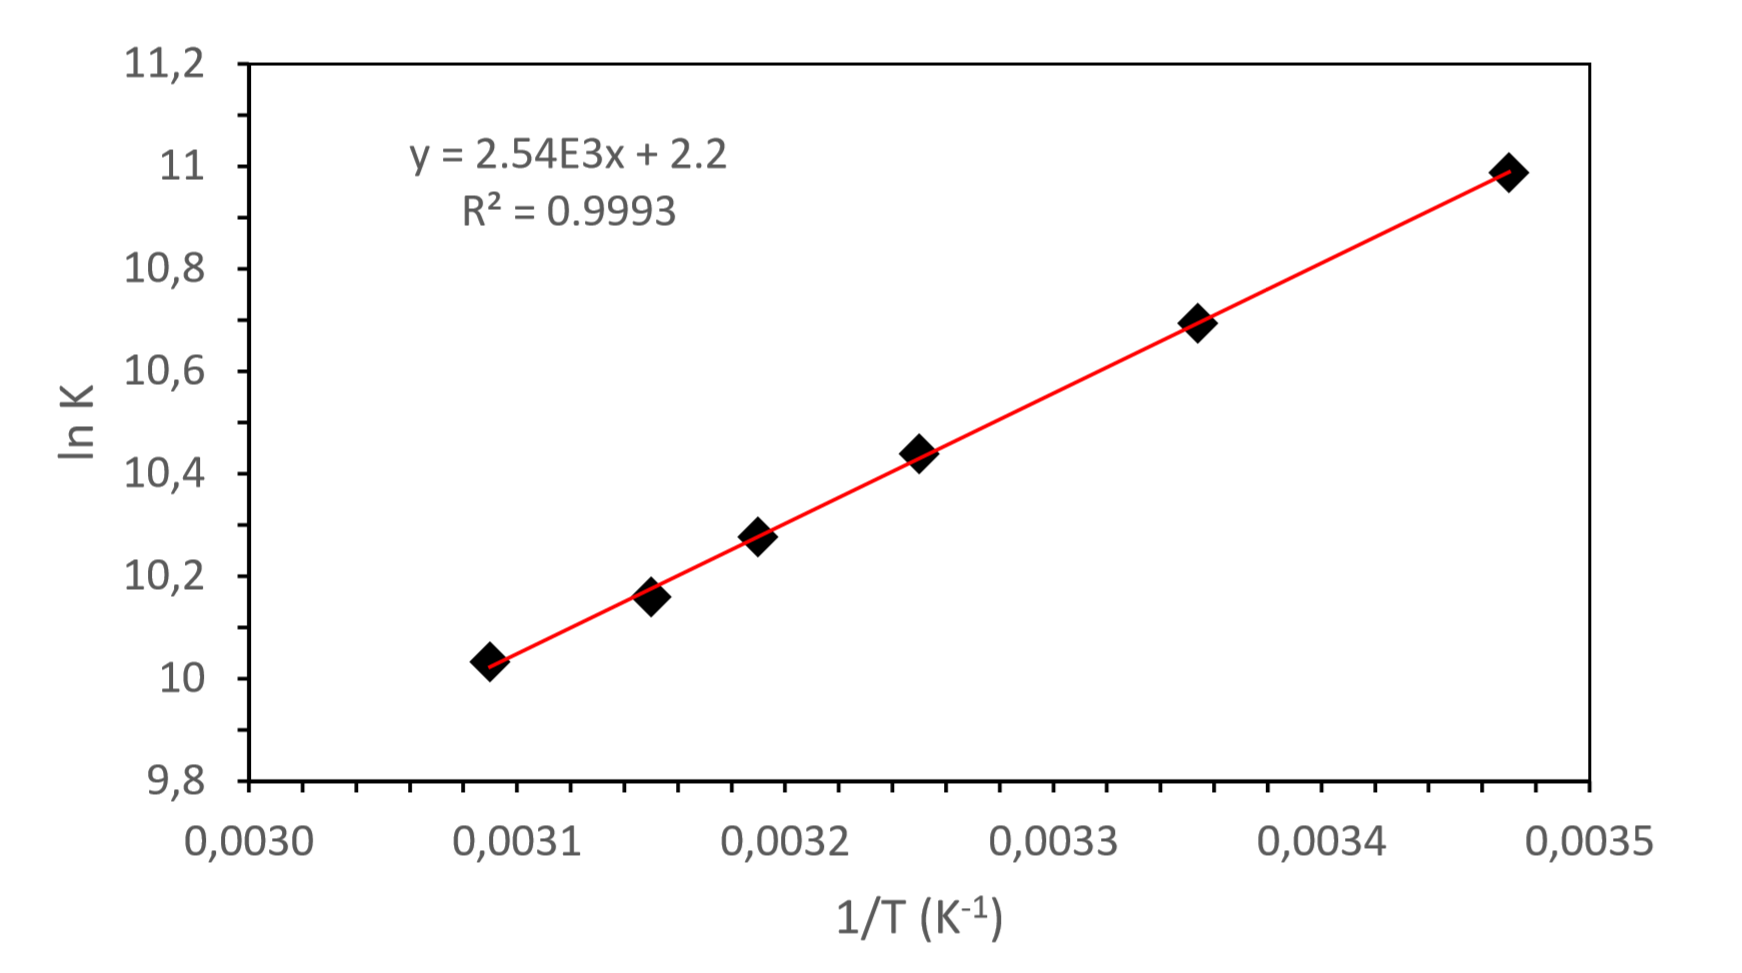
\includegraphics[width=14cm]{./pic/t24-1.png}
	% \caption*{从NaCl开始制备一些钠化合物。}
\end{figure}

\noindent\textbf{24.7.}
根据上图及 $K=e^{-\frac{\Delta  G}{RT}}$,计算25 °C下AO与DNA结合反应的$\Delta\mathrm{  _r}H^\circ$,$\Delta \mathrm{  _r}S^\circ$和$\Delta \mathrm{  _r}G^\circ$。(假设$\Delta \mathrm{  _r}H^\circ$和$\Delta \mathrm{  _r}S^\circ$不随温度变化)

AO在较高浓度下可发生自身聚集(二聚),其用于定量分析的二聚反应表达式为:

\[\ce{2D <=>[{k_\mathrm{f}}][{k_\mathrm{d}}] D_2 }\]

\noindent 其中\textbf{D}表示AO单体,\textbf{D}\(_2\)表示AO二聚体,$k_\mathrm{f}$和$k_\mathrm{d}$分别为二聚体生成和解聚的速率常数。根据上述反应,AO浓度与弛豫时间$\tau$(即反应体系中有突变后体系回到平衡需要的时间)有如下关系:

\[\frac{1}{\tau} = k_\mathrm{d} + 4k_\mathrm{f}\ c_\mathrm{AO}\]

\noindent 下表给出25 °C下AO二聚反应的数据:

\begin{longtable}[]{@{}ll@{}}
    \toprule
    10\textsuperscript{6} \emph{C}\textsubscript{AO} (mol
    dm\textsuperscript{--3}) & 10\textsuperscript{5} 弛豫时间 \emph{$\tau$}(
    s)\tabularnewline
    \midrule
    \endhead
    2.50 & 2.32\tabularnewline
    4.50 & 2.27\tabularnewline
    8.00 & 2.18\tabularnewline
    11.0 & 2.11\tabularnewline
    \bottomrule
\end{longtable}

\noindent\textbf{24.8.}
计算$k_\mathrm{d}$和$k_\mathrm{f}$的值。

不同浓度下(\(0\)至$\mathrm{7.3 \times 10^{-5} mol\ dm^{–3}}$)AO衍生物在水溶液中的吸收光谱如下图所示。光谱显示存在两个吸收峰,一个在496 nm,另一个在475 nm。图中右上角小图给出吸收峰强度之比(A\(_{475}\)/A\(_{496}\))与AO浓度的关系。

\begin{figure}[h]
	\centering
	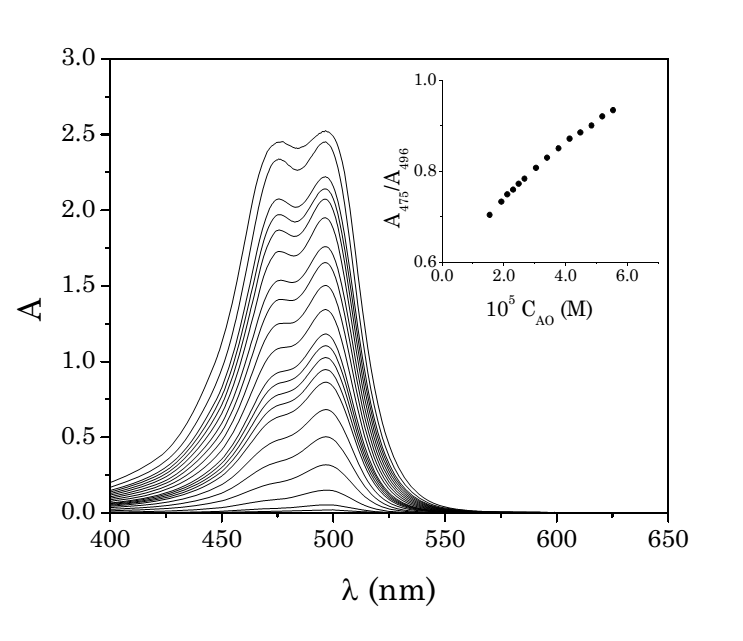
\includegraphics[width=14cm]{./pic/t24-2.png}
	% \caption*{从NaCl开始制备一些钠化合物。}
\end{figure}

\noindent\textbf{24.9.}
根据上述AO衍生物的吸收光谱图,选出以下正确的一(几)项:
\renewcommand{\labelitemi}{$\square$}
\begin{itemize}
    \item 496 nm的峰对应于单体形式。
    \item 如果只有单体形式,吸收峰强度之比(A\(_{475}\)/A\(_{496}\))会是常数。
    \item 为减少二聚,应当降低AO的浓度。
\end{itemize}
\renewcommand{\labelitemi}{$\bullet$}

\noindent\textbf{24.10.}
若AO初始浓度为$\mathrm{1.0 \times 10^{-5} mol\ dm^{-3}}$,计算平衡时AO二聚体的占比。

\[\ce{2D <=>[{k_\mathrm{f}}][{k_\mathrm{d}}] D_2 }\]
